\subsubsection{Red and Green LED Parallel Ports}

The red lights {\it LEDR}$_{17-0}$ and green lights {\it LEDG}$_{8-0}$ on the \DEBoard~board
are each driven by an output parallel port, as illustrated in Figure \ref{fig:LED_port}. The port
connected to {\it LEDR} contains an 18-bit write-only {\it Data} register, which has the
address {\sf 0xFF200000}. The port for {\it LEDG} has a nine-bit {\it Data}
register that is mapped to address {\sf 0xFF200010}. 
These two registers can be written using word accesses, and 
the upper bits not used in the registers are ignored.

\begin{figure}[h!]
   \begin{center}
       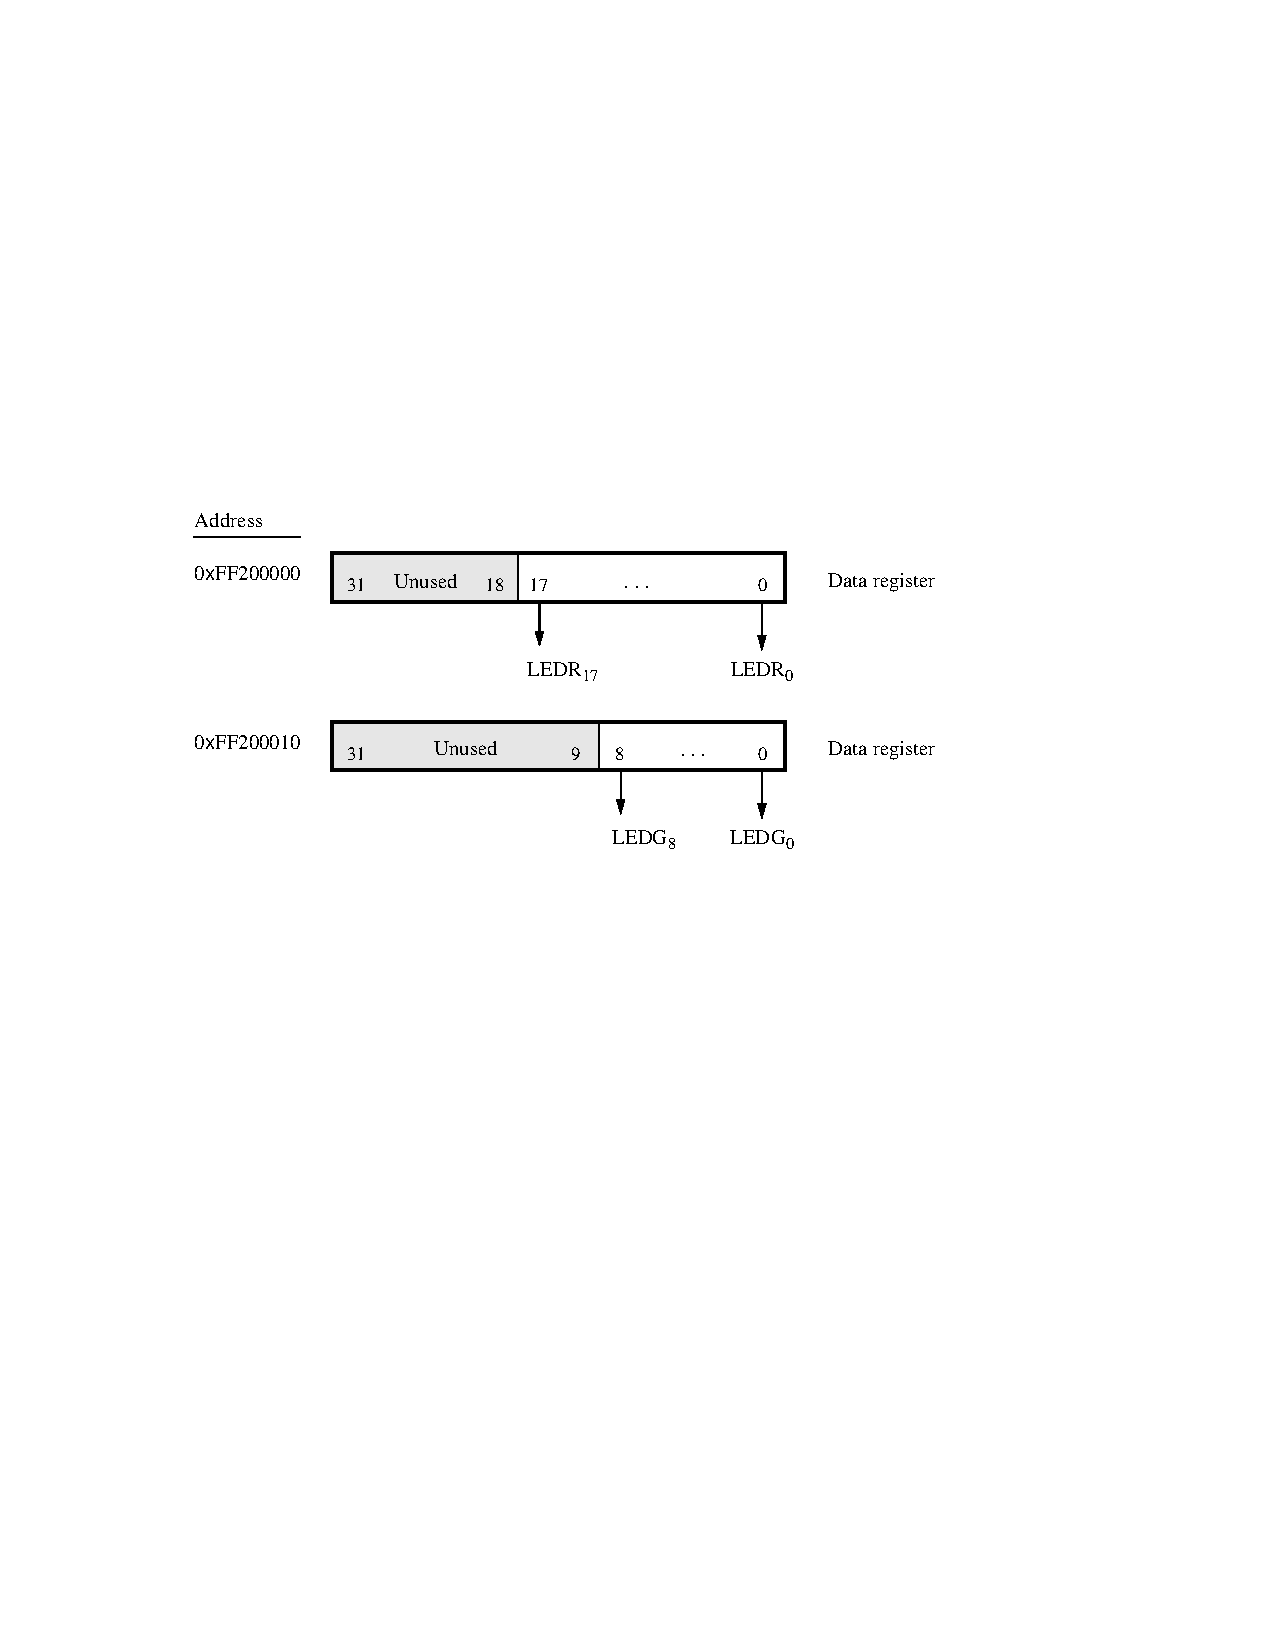
\includegraphics{../../../common/figs/FPGA_PP_Red_Green_LEDs.pdf}
   \end{center}
   \caption{Output parallel ports for {\it LEDR} and {\it LEDG}.}
	\label{fig:LED_port}
\end{figure}